\documentclass[conference]{IEEEtran}
\usepackage{amsmath,amssymb,booktabs,graphicx,tikz,cite,algorithmic,algorithm,url,microtype}
\usetikzlibrary{arrows.meta,positioning,fit,backgrounds}
\hyphenation{cal-i-bra-tion}
\newcommand{\hs}{\mathrm{HCCR}}
\begin{document}
\title{When Does Horizon-Specific Residual Calibration Change Advance Fleet Reservation? A Simulation Diagnostic of Coverage, Decisions, and Cost}
\author{\IEEEauthorblockN{Mainak Debnath, Krishna Chowdhary, Priyanshu Kumar}
\IEEEauthorblockA{Dept.\ of CSE (AI\&ML), Institute of Engineering and Management, Kolkata, India\\
\{Mainak.Debnath2023, Krishna.chowdhary2023, Priyanshu.Kumar2023.1\}@iem.edu.in}}
\maketitle

\begin{abstract}
Horizon-specific residual calibration (HCCR) changes the forecast-error scenarios behind advance vehicle reservation, yet rarely changes the reserve decision: HCCR and pooled calibration choose different reserve sets in 0.4--9.0\% of decisions per regime on average, so better coverage does not translate into proportional cost gains. In a synthetic multi-region simulation with strictly non-anticipative calibration (4 regimes, 30 seeds, horizons 1--28~d), averaged over $h\in\{1,7,14\}$, HCCR's cost advantage over pooling is small (0.1--0.5\% of HCCR's cost; up to 1.1\% on 30 replication seeds). It is largest at $h{=}1$ (AR: 2.2\%) and reverses at 14--28~d under persistent shocks (AR: $-$0.8\% and $-$2.5\%). Two pre-registered tests show that the reversal requires persistent residuals and depends on window freshness: staling only the pooled policy (deployable) shifts HCCR's relative cost by about $+0.10$ at $h{=}14$ and 28, removing nearly all of the $h{=}14$ reversal but about a fifth of the $h{=}28$ one. A descriptive check on 103 test days of public bike-sharing demand (one city, no routing) finds differences below 0.4\% of cost with inconsistent sign. Apart from that check all evidence is synthetic; no published method was re-implemented.
\end{abstract}
\begin{IEEEkeywords}
capacitated vehicle routing, demand forecasting, fleet reservation, residual calibration, predict-then-optimize
\end{IEEEkeywords}

\section{Introduction}
\textbf{Problem.} Advance fleet reservation must be committed before orders are confirmed: a vehicle reserved $h$ days ahead is paid for whether or not demand materialises, while demand beyond available capacity is unmet or unroutable. Forecasts therefore inform the reserve decision, and forecast uncertainty enters through scenarios of future demand. Prior work already couples demand prediction with advance rental and routing \cite{wei2024}, regional forecasts with vehicle loading \cite{armayau2026}, scenario-based hedging \cite{jia2025}, and two-stage fleet decisions with unmet-demand penalties \cite{beatrici2025}. We do \emph{not} claim a new reservation algorithm or solver.

\textbf{Puzzle.} Forecast-error distributions generally depend on the horizon, so estimating residuals per horizon (HCCR) instead of pooling them should give better-calibrated scenarios, and here it moves coverage toward nominal at most, but not all, horizons. But the reserve decision is a discrete choice among only 27 capacity steps, driven by the scenario tail near a quantile set by the cost-to-penalty ratio, so better-calibrated scenarios can leave the chosen set unchanged. Coverage, reserve-set choice, cost, unmet demand and routing feasibility are distinct outcomes.

\textbf{Research question.} When does horizon-specific residual calibration change advance reserve decisions, and when does that lower their cost?
\textbf{Hypothesis (pre-specified in the frozen configuration).} In regimes where error dispersion grows with horizon (AR, drift), HCCR has lower mean total cost than pooling over $h\in\{1,7,14\}$; in a horizon-invariant control (IID) the difference is zero.

\textbf{Evidence in brief.} HCCR and pooling choose different reserve sets in 0.4--9.0\% of decisions on average per regime (up to 17\% at single horizons); the cost advantage averaged over $h\in\{1,7,14\}$ is small and varied between seed sets; it reverses at 14--28~d under AR shocks; and two pre-registered tests show the reversal depends on persistent residuals and on window freshness, but leave most of the $h{=}28$ reversal unexplained (Sec.~V). \textbf{Scope.} The evidence is synthetic apart from one descriptive real-data check (single city, no routing); no published method was re-implemented; the closest papers were read in part (Sec.~II).

\textbf{Contributions.}
\begin{enumerate}
\item \emph{A controlled one-factor comparison of horizon-specific and pooled residual calibration.} With forecasts, costs, fleet and seeds matched, HCCR is cheaper than pooling over $h\in\{1,7,14\}$ in AR, Drift and Surge but not in the IID control (Table~\ref{tab:abl}, Table~\ref{tab:rep}). \emph{Boundary:} synthetic regimes, one forecaster family and assumed costs; the effect is small and not shown on real data. It would be refuted by CIs including zero in AR/Drift on new seeds or a non-zero IID effect.
\item \emph{A diagnostic link between coverage, decision change and cost.} Horizon-specific calibration moves coverage toward nominal at $h{=}1,14,28$ (still 0.73 at $h{=}28$ in AR) yet changes reserve sets in 0.4--9.0\% of decisions on average per regime, and its cost advantage is horizon-dependent, reversing at $h\ge14$ in AR; two pre-registered tests partly characterise the reversal. \emph{Boundary:} disagreement is descriptive (60 simulations per regime, unit = simulation) and reaches 14--17\% at single AR horizons; the mechanism remains partly unresolved. The claim would be refuted by horizon-invariant effects on new seeds or by high disagreement together with large cost differences.
\item \emph{A confirmed-order feasibility firewall.} Reserved, activated and routed states are kept separate so that forecast quantities never enter orders, demands, capacities or CVRP constraints, enforced by an interface without a forecast argument and 13 core automated invariant tests (28 tests with the mechanism scaffold; oracle exempt). \emph{Boundary:} a software invariant verified by tests on this implementation, not a proof, and not validated on operational data.
\end{enumerate}

\section{Related Work}
Wei et al.\ \cite{wei2024} decide additional rental in advance from demand prediction (abstract and highlights read only). Jia et al.\ \cite{jia2025} (read in part: the opening sections of the arXiv version) generate scenarios from multi-horizon quantile forecasts \cite{wen2017} and benchmark residual-based sample-average approximation \cite{kannan2022}, which they report matches quantile-based scenarios on simple patterns and trails on complex data. Kannan et al.\ \cite{kannan2022} (main text read) build scenarios from in-sample or leave-one-out regression residuals, optionally rescaled by an estimated covariate-dependent scale, with guarantees under i.i.d. or mixing/stationary conditions. In their terms, pooling residuals across horizons ignores heteroscedasticity and horizon-specific calibration uses the horizon as the scale covariate, so the idea behind our comparison is \emph{not} new; we add a rolling-origin, strictly non-anticipative time-series protocol, a discrete reservation objective and decision-level diagnostics, and we claim none of their guarantees for our serially dependent, non-stationary residuals. Beatrici et al.\ \cite{beatrici2025} (preprint) choose fleet size/mix with an unserved-demand penalty. Robust and conformal methods \cite{ghosal2024,patel2024} give guarantees under their own assumptions; time-series conformal guarantees need further conditions \cite{gibbs2021,barber2023}, and \emph{we claim none}. Decision-focused learning \cite{elmachtoub2022} and stochastic/dynamic routing surveys \cite{gendreau2016,psaraftis2016} frame the context. None of these methods was re-implemented here.



\section{Problem Formulation and Method}
\textbf{Notation.} Regions $r$, days $t$, demand $y_{r,t}$ (load units). A decision is made at origin day $d$ for target day $d{+}h$, $h\in\mathcal H=\{1,7,14,28\}$. Base capacity $A_r$ is fixed (here $\lceil\kappa\bar y_r\rceil$ from the first 400 days, $\kappa{=}1.05$).

\textbf{Forecast.} A direct-horizon seasonal linear regression (trend, weekly and annual Fourier terms, last observation, trailing 7-day mean; one OLS per $h$, refit weekly on targets already observed) gives $\hat y^{(h)}_{r,d}$; direct multi-step forecasting avoids recursive error accumulation \cite{chevillon2007}. Naive weekly-repeat and Holt--Winters are used in the forecaster ablation.

\textbf{Causal residual calibration.} (``Causal'' means non-anticipative, i.e.\ only information available at the decision time is used; it is not a causal-inference claim.) Define $e_{r,o,h}=y_{r,o+h}-\hat y^{(h)}_{r,o}$. Its value is observable only at day $o{+}h$. Hence at decision time $d$ the eligible set is $\mathcal E_{r,h}(d)=\{e_{r,o,h}: o_0\le o\le d-h\}$, truncated to the $W{=}200$ most recent. The pooled variant uses $\mathcal E_r(d)=\bigcup_{h'\in\mathcal H}\mathcal E_{r,h'}(d)$. Scenarios are $\tilde D_b=\max(0,\hat y^{(h)}_{r,d}+e_b)$, $e_b\in\mathcal E$. Note the \emph{information delay}: the window for horizon $h$ ends $h$ days before $d$.

\textbf{Reservation decision.} Reserve vehicle types $j$ (capacities $Q_j\in\{10,20,40\}$, at most two each, cost $c_j=4+0.5Q_j$) form 27 candidate sets $S$ with capacity $Q(S)$ and cost $c(S)$. With shortage penalty $\pi$ per unmet unit,
\begin{equation}
S^\star=\arg\min_{S}\; c(S)+\pi\,\tfrac1B\sum_{b=1}^{B}\big(\tilde D_b-A_r-Q(S)\big)_+ .
\label{eq:obj}
\end{equation}
Costs, $\pi{=}2$, and $\kappa$ were fixed before any test outcome was seen and are assumptions, not estimates from data.

\textbf{Horizon gate.} Policy $p$ acts at horizon $h$ only if its mean total cost on the validation window (origins 700--799) is below that of the reactive policy at $h$; otherwise it reserves nothing.

\begin{algorithm}[t]\caption{HCCR reserve decision at origin $d$ (reservation state only)}\label{alg:hccr}
\begin{algorithmic}[1]
\STATE \textbf{Input:} $\hat y^{(h)}_{r,d}$, past residuals with targets $\le d$, $A_r$, pool $(Q_j,c_j)$, $\pi$, gate $g_h$
\IF{$g_h=0$ or $|\mathcal E_{r,h}(d)|<30$} \RETURN $S=\emptyset$ \ENDIF
\STATE $\tilde D_b\gets\max(0,\hat y+e_b)$ for $e_b\in\mathcal E_{r,h}(d)$
\STATE $S^\star\gets\arg\min_S c(S)+\pi\,\mathrm{mean}_b(\tilde D_b-A_r-Q(S))_+$ \COMMENT{enumerate 27 sets}
\RETURN $S^\star$ \COMMENT{reserved, cost paid; \textbf{no order is created}}
\end{algorithmic}\end{algorithm}
\emph{Complexity:} $O(|\mathcal S|\,B)$ per decision ($27\times\le200$), plus one OLS per refit; no stopping criterion is needed because the search is exhaustive.

\textbf{Feasibility firewall.} Three states are kept separate (Fig.~\ref{fig:method}): \emph{reserved} (forecast-driven, cost paid), \emph{activated} (dispatcher rule using only confirmed demand $D$: the smallest-capacity subset of reserved vehicles with $A_r+Q\ge D$, else all), and \emph{routed} (the repository's OR-Tools service on exactly the confirmed orders with real vehicle capacities, 1\,s limit, first solution). Invariants, enforced by 13 automated tests: forecasts never create orders or change demands; the solver interface has no forecast argument; activation never exceeds the reserved set; decisions at $d$ are unchanged when all data after $d$ are altered (the oracle must change); calibration windows contain only realised targets.

\begin{figure*}[t]\centering
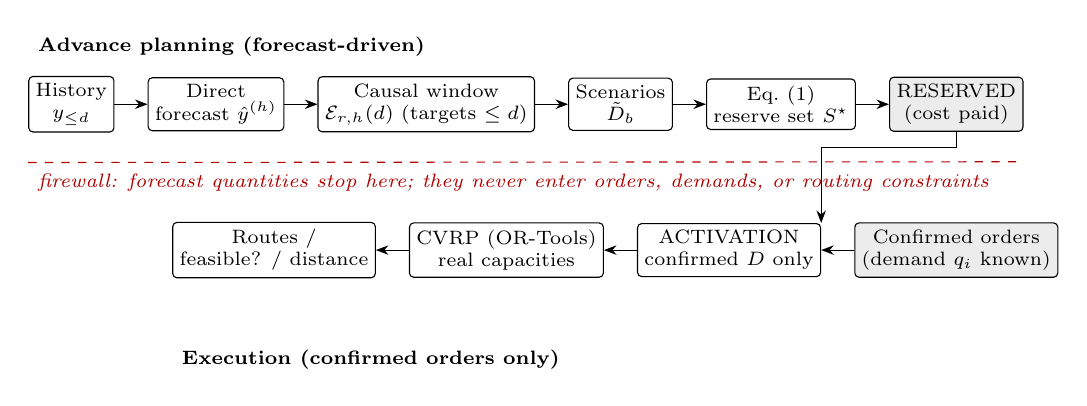
\begin{tikzpicture}[font=\scriptsize,node distance=0.42cm,box/.style={draw,rounded corners=1.5pt,minimum height=0.62cm,align=center,inner sep=2.5pt},fwd/.style={-{Stealth[length=1.6mm]},line width=0.4pt}]
\node[box](h){History\\$y_{\le d}$};
\node[box,right=of h](f){Direct\\forecast $\hat y^{(h)}$};
\node[box,right=of f](w){Causal window\\$\mathcal E_{r,h}(d)$ (targets $\le d$)};
\node[box,right=of w](s){Scenarios\\$\tilde D_b$};
\node[box,right=of s](o){Eq.~(1)\\reserve set $S^\star$};
\node[box,right=of o,fill=gray!15](rs){RESERVED\\(cost paid)};
\node[box,below=1.15cm of rs,fill=gray!15](oc){Confirmed orders\\(demand $q_i$ known)};
\node[box,left=of oc](ac){ACTIVATION\\confirmed $D$ only};
\node[box,left=of ac](cv){CVRP (OR-Tools)\\real capacities};
\node[box,left=of cv](rt){Routes /\\feasible? / distance};
\draw[fwd](h)--(f);\draw[fwd](f)--(w);\draw[fwd](w)--(s);\draw[fwd](s)--(o);\draw[fwd](o)--(rs);
\draw[fwd](rs.south)--++(0,-0.2)-|(ac.north east);\draw[fwd](oc)--(ac);\draw[fwd](ac)--(cv);\draw[fwd](cv)--(rt);
\draw[dashed,red!70!black] ([yshift=-0.38cm]h.south west) -- ([yshift=-0.38cm]rs.south east);
\node[red!70!black,anchor=north west,font=\scriptsize\itshape] at ([yshift=-0.40cm]h.south west){firewall: forecast quantities stop here; they never enter orders, demands, or routing constraints};
\node[anchor=north west] at ([yshift=0.62cm]h.north west){\textbf{Advance planning (forecast-driven)}};
\node[anchor=north west] at ([yshift=-0.78cm]rt.south west){\textbf{Execution (confirmed orders only)}};
\end{tikzpicture}\caption{Method and firewall. Only the reserved set crosses from planning to execution; activation and routing use confirmed demand.}\label{fig:method}\end{figure*}

\section{Experimental Setup}
\subsection{Audit of the predecessor artifacts}
The predecessor manuscript's Table~II (naive/Holt--Winters/LR MAPE of 21.29/12.48/8.02\%) could not be reproduced: 40 seeds of the repository implementation give LR 60-day MAPE of 2.95--6.20\% and naive 7.86--13.75\%, and its error growth with horizon is absent under rolling-origin evaluation (LR MAE 4.58/4.71/4.79/4.55 at 7/14/30/60 d). Its original setup was not recorded, so this shows only that the numbers cannot be attributed to the repository code. We use none of them.

\subsection{Data: synthetic simulator (not real observations)}
Four regions (levels 80/100/120/90), $T{=}1100$ days: $L_r(1+0.0002t+0.12\sin(2\pi t/7{+}\phi_r)+0.10\sin(2\pi t/365.25{+}\psi_r))$ plus noise (5\% of level). Regimes add: \textbf{IID} nothing (null control: error independent of horizon); \textbf{AR} latent AR(1), $\phi{=}0.95$, sd 10\%; \textbf{Surge} unforecastable 3-day surges (prob.\ 0.01/day, +30--80\%); \textbf{Drift} random-walk level (sd 0.8\%/day). Splits: days 0--399 initial fit, 400--699 calibration, 700--799 validation (buffer and gate selection), origins 800--1071 test (272 origins $\times$ 4 regions $\times$ 4 horizons per seed). Seed counts differ by experiment because of compute cost, and were fixed in the frozen configuration before analysis: 30 per regime for the main comparisons, 10 for the forecaster ablation (Holt--Winters fitting) and routing (OR-Tools solves, 6 instances per seed), 15 for the nine sensitivity configurations; there was no formal power analysis.

\subsection{Policies, metrics, statistics}
All policies share forecasts, scenarios, costs, splits and seeds: \textbf{Reactive} (reserve nothing); \textbf{Point} (Eq.~\ref{eq:obj} with $B{=}1$ at $\hat y$); \textbf{Buffer} (cheapest set covering $\hat y+b_h$, $b_h$ chosen per horizon on validation from a fixed grid); \textbf{Pooled}; \textbf{HCCR}; \textbf{Robust} (cheapest set covering $\hat y$ plus the 95th percentile of horizon-specific residuals; conservative, no cost model; its 0.95 quantile was fixed a priori and, unlike the buffer, not validation-tuned, so it is a conservative reference rather than an optimised competitor); and an \textbf{Oracle} (Eq.~\ref{eq:obj} with the true $y$; unattainable). Gating applies identically to every non-reference policy so that each ablation changes exactly one component of HCCR: B pooling scope, C calibration, D objective, E gate, F forecaster. Metrics per decision: reservation cost $c(S)$; unmet demand $u=(y-A_r-Q(S))_+$; total cost $C=c(S)+\pi u$; shortage-day rate $\mathbb 1[u>0]$; reserved vehicles. Routing metrics (10 seeds/regime, 6 random outcome-blind instances per seed, $h{=}7$, same orders and coordinates for every policy): feasibility $=\mathbb 1[\text{all confirmed orders served}]$; distance only over solved instances, never zero-filled. Statistical unit: the simulation, i.e.\ (regime, seed), with regions and days averaged inside it; 95\% percentile-bootstrap CI (10\,000 resamples) of paired differences $\Delta=C_{\text{comparator}}-C_{\hbox{\scriptsize HCCR}}$ ($\Delta{>}0$: HCCR cheaper), Wilcoxon signed-rank, Holm correction over the 20 confirmatory tests (5 comparisons $\times$ 4 regimes at $h\in\{1,7,14\}$), and $d_z$. Only the 20 confirmatory tests of Table~\ref{tab:abl} are Holm-corrected; CIs in Tables~\ref{tab:pol}, \ref{tab:mod} and \ref{tab:sens} are uncorrected and descriptive. Interval metrics use the central 80\% residual interval; no coverage guarantee is claimed.

\section{Results}
\subsection{Forecast accuracy and calibration (reported separately)}
The regimes behave as designed (Fig.~\ref{fig:results}): WAPE of the point forecast grows from 4.6\% at $h{=}1$ to 8.3\% at $h{=}28$ (AR) and 3.8\% to 5.3\% (Drift), and is flat for IID (3.4\%) and Surge (4.8--4.9\%). In AR, pooled 80\% intervals over-cover at $h{=}1$ (0.90) and under-cover at $h{=}28$ (0.68); horizon-specific intervals are closer to nominal at $h{=}1,14,28$ (0.79, 0.76, 0.73) but still under-cover at long horizons, and at $h{=}7$ pooling is closer in AR and Drift (0.788 vs.\ 0.777; 0.805 vs.\ 0.783). We therefore claim improved, not corrected, coverage. Coverage and cost are distinct outcomes: coverage scores a central 80\% interval, whereas Eq.~\eqref{eq:obj} depends on the tail of $\tilde D$ near the quantile set by the cost/penalty ratio and then rounds to one of only 27 capacity steps. \emph{Decision disagreement} (all 30 primary and all 30 replication simulations per regime; share of test decisions at which the two policies choose different reserve sets; unit = simulation; ungated decisions, gated ones are nearly identical) averages 0.4\% (IID), 3.6\% (Drift), 3.8\% (Surge) and 8.3\% (AR; 95\% CI 7.4--9.1; replication 9.0\%) over $h\in\{1,7,14\}$. It is not uniformly below 10\%: in AR it is 14.0\% at $h{=}1$ and 17.4\% at $h{=}28$ (CIs 12.6--15.4 and 15.6--19.4), i.e.\ highest at the two horizons where the cost effects have opposite signs. Better calibration therefore does not by itself imply better reservation.

\subsection{Baseline comparison}
\begin{table*}[t]\centering\caption{Quantitative comparison under identical forecasts, confirmed demand, costs and seeds; mean over regimes and $h\in\{1,7,14\}$ (model cost units). Cost CI: 95\% bootstrap over 120 (regime, seed) simulations. Route feasibility: $h{=}7$, 240 instances per policy, CI over 40 simulations. Point-forecast WAPE is shared by all policies (4.6\%, seasonal LR). Per-regime and per-horizon versions: \texttt{comparison\_table.csv}.}\label{tab:pol}
\footnotesize\setlength{\tabcolsep}{4pt}
\begin{tabular}{lcrrrrc}\toprule
Policy & Total cost [95\% CI] & Reserve cost & Unmet units & Shortage-day rate & \#Veh.\ reserved & Route feas.\ \% [CI]\\\midrule
\input{assets/tab_comparison_rows}\\\bottomrule
\end{tabular}\end{table*}
Table~\ref{tab:pol} shows that point, buffer, pooled and HCCR policies cut mean total cost by 43--46\% relative to reactive routing (per-regime cuts for HCCR: 40--54\%), which mainly reflects our assumption that a missing unit costs more than a reserved one; it is not evidence of real-world benefit. The conservative robust cover cuts it by only 19\%: ungated it over-reserves (mean cost 18.3 with almost no unmet demand), and the validation gate frequently reverts it to reactive (gate open in 28--89\% of seeds by regime); the ungated reference row isolates the gate's effect. Marginal CIs of HCCR, point and pooled overlap; this is not a test of equality, and the paired comparisons below are the proper evidence. The oracle is 1.6--3.6 cost units cheaper than HCCR, far larger than any difference among calibration variants. Routing feasibility ranks differently from cost: the fixed buffer (69.6\%) exceeds the oracle (60.4\%), because Eq.~\eqref{eq:obj} is defined on aggregate capacity while indivisible orders need slack; among instances whose aggregate capacity sufficed, 10--21\% of outcomes were still unroutable (7 of 70 for reactive, 39 of 184 for the oracle).

\subsection{Ablation (single-factor)}
\begin{table*}[t]\centering\caption{Paired cost differences $\Delta$ (comparator $-$ HCCR) over $h\in\{1,7,14\}$, mean [95\% bootstrap CI]; $^\ast$ Holm-adjusted $p<0.05$. Positive: HCCR cheaper. Last rows: pooled vs.\ HCCR by horizon.}\label{tab:abl}
\footnotesize\setlength{\tabcolsep}{3pt}
\begin{tabular}{lcccc}\toprule
Comparator (removed component) & IID & AR & Surge & Drift\\\midrule
\input{assets/tab_ablation_rows}\\\midrule
\input{assets/tab_ablation_byh_rows}\\\bottomrule
\end{tabular}\end{table*}
Table~\ref{tab:abl} gives the ablations. \textbf{B} (pooling): indistinguishable from zero in the IID control (mean $-$0.0003 [$-$0.003, +0.002]; a CI, not a proof of equivalence); small but Holm-significant gains in AR (+0.08, $d_z{=}1.14$), Surge (+0.01) and Drift (+0.04), i.e.\ 0.5\%, 0.1\% and 0.3\% of HCCR's own cost averaged over the three horizons, but 2.2\% (AR) at $h{=}1$. The by-horizon rows show why the average is small: HCCR wins at $h{=}1$ in AR (+0.29) but loses at $h{=}14$ ($-$0.12) and $h{=}28$ ($-$0.42), with CIs excluding zero. A plausible (untested) explanation is the information delay: the horizon-$h$ window ends $h$ days earlier and is autocorrelated under persistent shocks. \textbf{C} (point forecast): small gains of 0.07--0.24, so most of the benefit of cost-aware reservation is already obtained from the point forecast. \textbf{D} (buffer): 0.56--0.87 in HCCR's favour on total cost, although the buffer buys higher routing feasibility. \textbf{E} (gate): exactly zero at $h\le14$; the gate never closed for HCCR at these horizons in the primary setting (it closed in 1 of 30 AR seeds at $h{=}28$), so the data do \emph{not} support the 14-day gate; the sensitivity runs show it can hurt. \textbf{F} (forecaster): see Sec.~V-E. \textbf{G} (firewall): by construction and by test, solver inputs contain no forecast; the same confirmed orders and fleet gave identical routing results.

\textbf{Hypothesis outcome.} At the primary horizons the data agree with the pre-specified direction in AR and Drift and with the null in IID, but the effects are practically negligible, and the by-horizon reversal at $h\ge14$ (AR) is not predicted by the hypothesis. A small gain also appears in Surge (+0.01), a regime where dispersion does not grow with horizon; we have no tested explanation and treat it as exploratory. The fixed buffer is the main trade-off: it costs 0.66 more than HCCR on the shared objective yet reserves more (0.91 vs.\ 0.66 vehicles), leaves less unmet demand (1.09 vs.\ 1.62) and routes more instances (69.6\% vs.\ 62.1\%); because we define no joint metric combining cost and routing feasibility, we do not declare either preferable.

\begin{table*}[t]\centering\caption{Replication of the primary contrast (pooled $-$ HCCR, mean over $h\in\{1,7,14\}$): original seeds 0--29 vs.\ independent seeds 100--129 (same frozen configuration), mean [95\% bootstrap CI]; columns 4--5 give original / replication values as \% of HCCR cost and the replication's $h{=}1$ / $h{=}28$ differences.}\label{tab:rep}
\footnotesize\setlength{\tabcolsep}{5pt}
\begin{tabular}{lcccc}\toprule
Regime & Seeds 0--29 & Seeds 100--129 & \% HCCR & $h{=}1$ / $h{=}28$\\\midrule
\input{assets/tab_rep_rows}\\\bottomrule
\end{tabular}\end{table*}
\textbf{Independent replication.} Direction replicates (IID null; AR gain at $h{=}1$ and loss at $h\ge14$), but magnitude does not: the averaged AR gain is 0.88\% of HCCR's cost (0.53\% originally) and Drift 1.08\% with a wide CI (0.04--0.32; 0.29\% originally), so we report the effect as small, sign-reversing in horizon, and \emph{not} bounded by 0.5\%. The replication was run once with the frozen configuration; its $p$-values are uncorrected.

\begin{figure}[t]\centering\includegraphics[width=0.97\columnwidth]{assets/fig_results.pdf}\caption{Empirical coverage of the central 80\% interval by horizon, horizon-specific (solid) vs.\ pooled (dashed) residuals, mean over 30 simulations per regime. Per-horizon cost differences are in Table~\ref{tab:abl} (last rows).}\label{fig:results}\end{figure}



\subsection{Mechanism test of the long-horizon reversal (pre-registered)}
\emph{Design (frozen and hashed before any run; a 30-simulation pilot served only for sample-size planning).} AR regime, latent persistence $\phi\in\{0.95,0\}$ at fixed stationary latent sd, calibration window $\in$ \{natural; \emph{anticipative}\} and $h\in\{14,28\}$, 60 fresh simulations (seeds 300--359, common random numbers). The anticipative window ends at $d{-}1$ and so uses future demand: it is a \emph{non-deployable diagnostic}. Primary contrast $\Theta_h=[\Delta^{\mathrm{ant}}_h-\Delta^{\mathrm{nat}}_h]_{\phi=0.95}-[\Delta^{\mathrm{ant}}_h-\Delta^{\mathrm{nat}}_h]_{\phi=0}$ (Holm over $h\in\{14,28\}$; minimum meaningful effect 0.10, a design choice).
\begin{figure}[t]\centering\includegraphics[width=0.97\columnwidth]{assets/fig_mechanism.pdf}\caption{Paired $\Delta$ (pooled $-$ HCCR) by window condition and persistence, mean with 95\% bootstrap CI over 60 simulations; open crosses = non-deployable diagnostic.}\label{fig:mech}\end{figure}
\emph{Results.} $\Theta_{28}=+0.32$ [0.28, 0.37] (Holm $p<0.001$); $\Theta_{14}=+0.03$ [0.01, 0.05] (Holm $p=0.006$, below the 0.10 minimum). At $\phi{=}0.95$ anticipation moves $\Delta_{28}$ from $-$0.445 to $-$0.112 [$-$0.173, $-$0.054]: most, not all, of the reversal; at $\phi{=}0$, $\Delta\approx0$ at every horizon, but $\phi$ also changes how residual dispersion grows with horizon (a declared confound). \emph{A pre-registered prediction failed:} adding 7/14/28 days of staleness to \emph{both} policies leaves $\Delta_1$ unchanged (0.294 $\to$ 0.314), so staleness alone is not the mechanism; the pattern fits \emph{relative} freshness (pooled windows contain fresh short-horizon residuals), which we did not test directly. Our pre-registered $h{=}1$ sanity check was mis-specified (pooled windows leak at $h{=}1$), so $\Theta_1\neq0$ by construction. Windows of 100/400 give $\Delta_{28}=-0.726/-0.303$ (vs.\ $-$0.445 at 200), so effective sample size matters; a 64-set fine pool raises disagreement at $h{=}28$ from 18\% to 75\% but not the reversal ($\Delta_{28}=-0.466$; costs differ), so quantisation explains the low disagreement, not the reversal.

\subsection{Relative-freshness test (second pre-registration)}
Experiment~1 left open why staleness \emph{per se} did not matter. We tested the hypothesis that pooled windows win at long horizons because they contain fresh short-horizon residuals, with a \emph{deployable} intervention: age \emph{only} the pooled policy's calibration information by $S$ days (HCCR, forecasts, demand and costs unchanged). Pre-registered contrast $\Psi_h=[\Delta_h(S{=}28)-\Delta_h(\text{natural})]_{\phi=0.95}-[\,\cdot\,]_{\phi=0}$, 45 fresh simulations (30-simulation pilot for variance only; $N$ from the pre-set power rule $\times1.5$). Results: $\Psi_{14}=+0.097$ [0.065, 0.131] and $\Psi_{28}=+0.096$ [0.061, 0.131] (Holm $p<0.001$), at the 0.10 minimum meaningful effect. At $\phi{=}0.95$ staling pooled moves $\Delta_{14}$ from $-$0.125 to $-$0.019 (nearly all of the reversal) but $\Delta_{28}$ only from $-$0.508 to $-$0.406 (about a fifth); at $\phi{=}0$ nothing changes. Relative freshness is thus supported but incomplete; the persistence/dispersion confound remains.

\subsection{Descriptive real-data check (third pre-registration)}
Public UCI Bike Sharing data (Capital Bikeshare, Washington D.C., 731 days, CC BY 4.0; obtained from a GitHub mirror, integrity-checked) were split into four hour-of-day \emph{segments} (not regions; resampled jointly because they share weather) with the same forecaster, 27-set pool, policies and a non-anticipative split (365 fitting days; test origins 600--702; $W{=}150$, a declared deviation). Counts are fulfilled rentals, so demand is supply-censored; there are no capacities or orders, so \emph{no routing is evaluated}. Costs are normalised scenario costs over $\pi\in\{1,2,4,9,19\}$ (primary 4). Across all 20 horizon$\times\pi$ cells, $|\Delta|$ is at most 0.33\% of HCCR's cost (threshold 1\%), its sign is inconsistent and most 28-day block-bootstrap CIs include zero; disagreement is 2.9--16.5\%. Unlike the simulation, horizon-specific intervals did not improve coverage (0.757 vs.\ 0.762 pooled at $h{=}1$; both under-cover), and forecasts are weak (WAPE 20--27\%). One city, one realisation: this is a consistency check, not validation.

\subsection{Forecaster and sensitivity analysis}
Seasonal LR has the lowest WAPE and HCCR cost in every regime (10 seeds per regime; \texttt{forecast\_model\_ablation.csv}); this is expected because the simulated structure matches its features and is not a claim about real demand. Paired against LR, Holt--Winters costs more in IID (+0.23), Surge (+0.94) and Drift (+0.10) with CIs excluding zero, but not in AR (+0.04 [$-$0.15, +0.20]); the weekly naive forecaster is worst (+0.70 to +1.66). Lower forecast error and lower operational cost coincided here, but the two were measured separately and need not do so in general.

Sensitivity runs (15 seeds per regime, regimes pooled; \texttt{sensitivity\_summary.csv}) vary the penalty $\pi$, reserve-cost scale, capacity pressure $\kappa$ and demand noise. The saving versus reactive routing swings from 1.8 ($\pi{=}1$) to 34.4 ($\pi{=}4$), so any headline saving is dominated by the assumed cost ratio. HCCR's advantage over pooling stays small and positive (+0.02 to +0.09) except at doubled noise, where it is indistinguishable from zero ($-$0.00 [$-$0.14, +0.08]). Its advantage over the point forecast disappears when capacity is ample ($\kappa{=}1.2$: $-$0.02 [$-$0.10, +0.03]). The validation-based gate was never beneficial and was harmful at $\kappa{=}1.2$, where the ungated policy was cheaper by 0.16 [0.06, 0.29]. Interpreting ablation E, the gate rule is therefore not supported by these experiments.

\section{Limitations and Conclusion}
\textbf{Baselines.} Implemented: the seven policies and naive/Holt--Winters forecasters under the HCCR objective. \emph{Not} implemented: Wei et al.'s joint rental--routing method, Jia et al.'s learned-quantile scenarios, Kannan et al.'s ER-SAA (the pooled policy is only conceptually similar), conformal or distributionally robust methods; no comparison to them is made. \textbf{Scope.} All evidence is simulated; regime parameters, costs and capacity pressure are assumptions, regions are independent, and one forecaster family dominates. Reported savings versus reactive routing depend on the assumed cost ratio and must not be read as field benefit. The robust cover was evaluated in the main and routing experiments only (the forecaster and sensitivity runs cover the other six policies). Routing was evaluated on a small outcome-blind sample with a first-solution solver (1\,s). The mechanism of the long-horizon reversal is only partly resolved (Sec.~V-D,E): the anticipative window is non-deployable, persistence is confounded with dispersion growth, freshness explains about a fifth of the $h{=}28$ reversal, and one regime family was tested. The real-data check is a single dataset (one city, supply-censored counts, segments instead of regions, no routing) with a shortened window; it does not validate operational benefit. We claim no conformal or distribution-free coverage. The predecessor manuscript's reported numbers could not be reproduced and are not used.

\textbf{Conclusion.} HCCR is a composition of known components. In this simulation study its horizon-specific calibration moves coverage toward nominal (not fully: 0.73 at $h{=}28$ in AR) but gives only marginal, horizon-dependent operational gains over pooling whose size varied between seed sets (0.1--1.1\% of HCCR's cost), stays well above the oracle's cost, and routing feasibility needs slack that a capacity-level objective does not provide. Validation on real order and fleet histories remains the necessary next step.

\textbf{Reproducibility.} From the repository root: \texttt{python -m research\_hccr.run\_study --stage all}, then \texttt{research\_hccr.analysis}, \texttt{comparison}, \texttt{diagnostics\_full}, \texttt{replication}, \texttt{mechanism.runner} and \texttt{mechanism.analyze}, \texttt{make\_assets}, and \texttt{verify\_claims} (122 checks of every number quoted here against the CSVs); tests: \texttt{pytest research\_hccr/tests}. The mechanism pre-registration and its SHA-256 are released. Stages ran in resumable chunks, not as one uninterrupted invocation.

\bibliographystyle{IEEEtran}
\bibliography{references}
\end{document}
